\chapter{Experimental results}

\section{Implementation details}
We implemented as a Python framework the whole architecture that has been described so far.

The code of the project can be divided into 3 parts.
\begin{itemize}
  \item The \textbf{model}: it contains the code of the physical model. The latter must be \textit{differentiable} and should comply with some internal API in order to be integrated effortlessly inside the rest of the library;
  \item the \textbf{NNs architecture}: it is the core of the project and it is configurable only via a defined API;
  \item the \textbf{experimental setup}: it is the code where the user can tweak all the parameters and decide how to test the chosen model.
\end{itemize}

\begin{figure}[H]
	\centering
	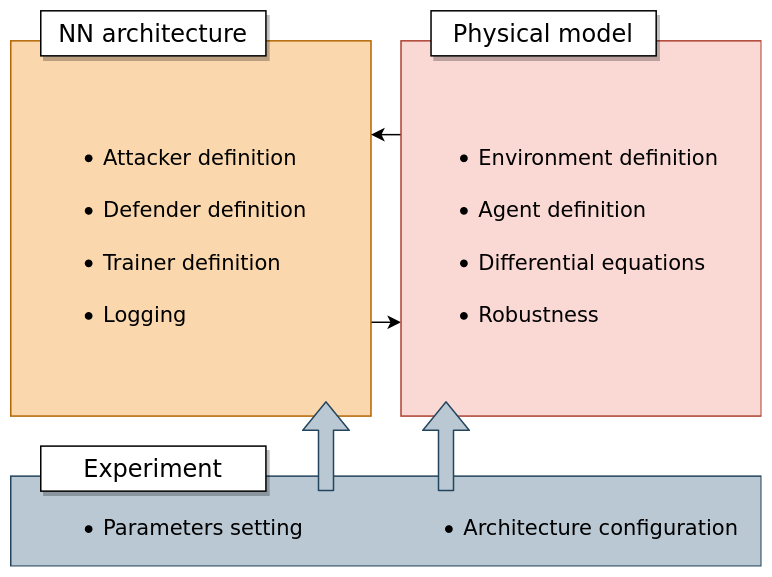
\includegraphics[width=10cm, keepaspectratio]{img/5_1_module_api.png}
	\caption{Schematic visualization of the interaction between the three main module of the architecture. The structure reflects the organization of the code as well.}
\end{figure}

In order to compute the robust semantics of the STL formulas in a fast and efficient way, it has been implemented a small separate module that parses and transforms the STL requirements into executable code.

The whole project relies extensively on PyTorch \cite{pytorch}, a Python library tailored to build complex numerical models.
All the computations leverage the PyTorch's computational graph, which eased the implementation and made the training of the NNs possible.
Unfortunately, due to the iterative nature of the training process, porting it on GPU did not provide benefits. In this regards there is room for improvements.


\section{Cruise control}
The problem of the cruise control has been described in the previous section: given a vehicle that moves along a road, the controller should be able to keep its velocity constant regardless of the steepness of the road.

\subsection{Experimental settings}
For the desired constant velocity, we fixed as \textit{setpoint} $\tilde{v} = 5 \frac{m}{s}$ and a tolerance $\varepsilon = 0.25 \frac{m}{s}$.
Therefore, the \textbf{constraint} applied to the velocity $v_c$ of the moving car $c$, is $\Phi = \mathcal{G}(v_c \leq 5.25 \wedge v_c \geq 4.75)$.

Due to the nature of the problem, the attacker controls the generation of the steepness of the road.
Such operation takes place \textbf{once}, at the beginning of each episode.

The \textbf{attacker}'s architecture has 2 layers with 10 neurons each.
To each layer is applied the \textit{Leaky ReLU} activation function \cite{xu2015empirical}.
The input noise vector $\textbf{z}$ belongs to the space $\mathbb{R}^5$.
This NN does not have other input since the \textit{environment} (the road) is a static object with no knowledge about the setting.
The output of the NN is the vector $\textbf{u}_\beta = (\pmb{\omega}, \pmb{\sigma})$ used to determine the function of the elevation of the road $r(x)$.
The dimension $d$, that defines the number of \textit{RBFs} composing $r(x)$, has been fixed to 3.

Since the environment is static and does not need to describe a dynamic behaviour, the \textit{policy function} of the attacker is defined over the space $\mathbb{R}^1$.

The \textbf{defender} NN has 3 layers with 10 neurons each.
To each layer is applied the {Leaky ReLU} activation function.

The \textit{defender} NN uses a \textit{policy function} defined over the space $\mathbb{R}^3$, due to the need of adapting and forecasting different scenarios.

The \textbf{initial configuration} of each training episode is sampled from an \textit{hyper-grid} of two dimensions: initial position $x_{c0}$ and initial velocity $v_{c0}$.
The initial position $x_{c0}$ is sampled uniformly from the interval $[0 \; m, 50 \; m]$.
Such choice has been made to introduce variability in the training and force the NNs to explore different strategies.
The initial velocity $v_{c0}$ is sampled among 25 equispaced points between $[-12 \frac{m}{s}, 12 \frac{m}{s}]$.

\begin{figure}[H]
	\centering
	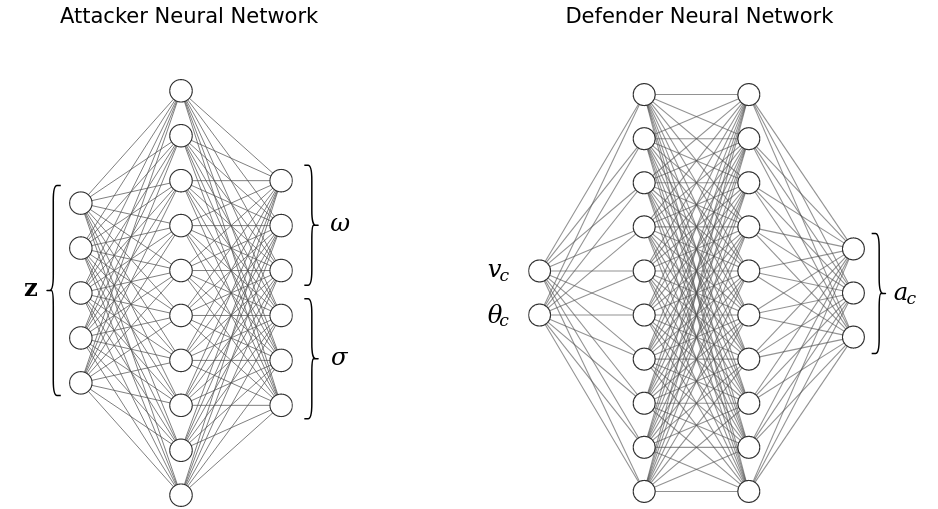
\includegraphics[width=12cm, keepaspectratio]{img/5_2_NNcruisecontrol.png}
	\caption{The architecture used for the the two NN in the cruise control case study. The \textbf{attacker} takes as input the noise vector $\textbf{z}$, while the output are the two vectors $\pmb{\omega}$ and $\pmb{\sigma}$ that characterize the . The \textbf{defender} takes as input the car's velocity $v_c$ and the inclination of the car (steepness) $\theta_c$ to compute the acceleration $a_c$.}
\end{figure}

During the training the \textbf{timestep} $\Delta t$ between two time instant has been set to $0.05s$ while the horizon $h$ for each episode was $500ms$, 10 timesteps.
The same \textit{timestep} has been used also in the testing.

The training phase lasted $30k$ \textit{cycles} and each \textbf{episode} has been repeated only 1 time for the \textit{attacker} and 10 times for the \textit{defender}.

\subsection{Metrics and results}
The testing configurations is the same of the training except for the the initial position $v_{c0}$ of the car, that is always assumed to be $0 \; m$.

We decided to test the model in three different scenarios.
In the first scenario the road is generated by the attacker NN by means of the \textit{RFBs}.
They create more complex shapes and produce realistic road profiles, this make them perfectly suitable for training but less suitable for assessing the performance of the controller.

In the second and third scenarios we have a flat landscape and, respectively, only one hill and only one valley.
Such simple tests are good to identify the pitfalls of the trained model.

In each figure we show the elevation of the road, the velocity of the car and the acceleration provided by the \textit{defender}.

\begin{figure}[H]
	\centering
	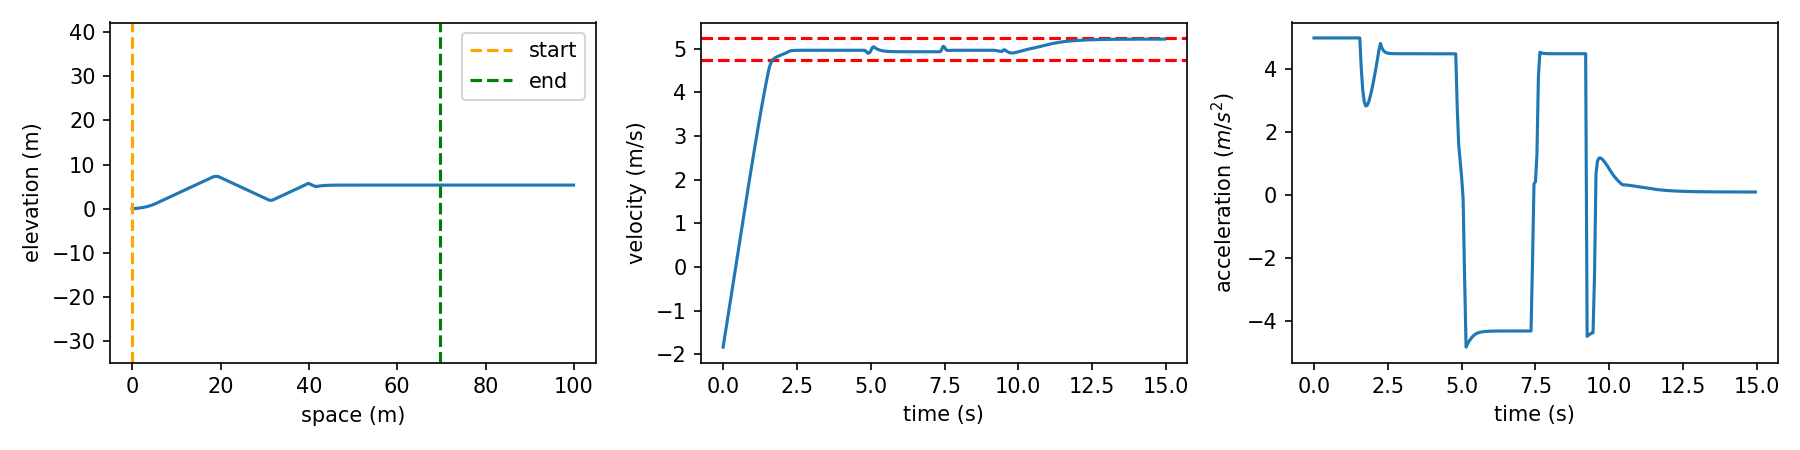
\includegraphics[width=13.8cm, keepaspectratio]{img/5_2_triplot_atk.png}
	\caption{Initial configuration: $v_{c0}=-2.04 \frac{m}{s}$. The model manages to reach the area of the desired velocity even starting from afar. Looking at the acceleration, it is possible to notice the adaptation of strategy in presence of a sudden change of steepness.}
    \label{fig:cruise_atk}
\end{figure}

\begin{figure}[H]
	\centering
	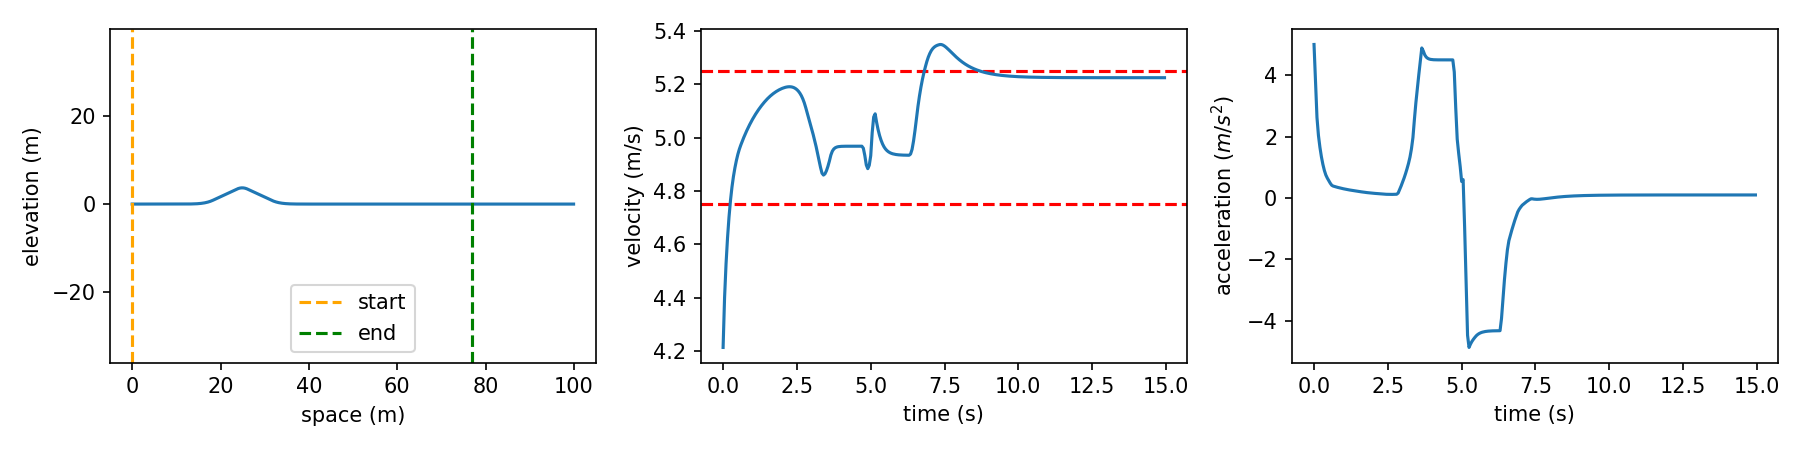
\includegraphics[width=13.8cm, keepaspectratio]{img/5_2_triplot_up.png}
	\caption{Initial configuration: $v_{c0}=3.96 \frac{m}{s}$. Here the car start with a velocity that is quite close to the setpoint. However, the trajectory presents a bit of overshoot in the correction that takes place right after the descent.}
    \label{fig:cruise_up}
\end{figure}

\begin{figure}[H]
	\centering
	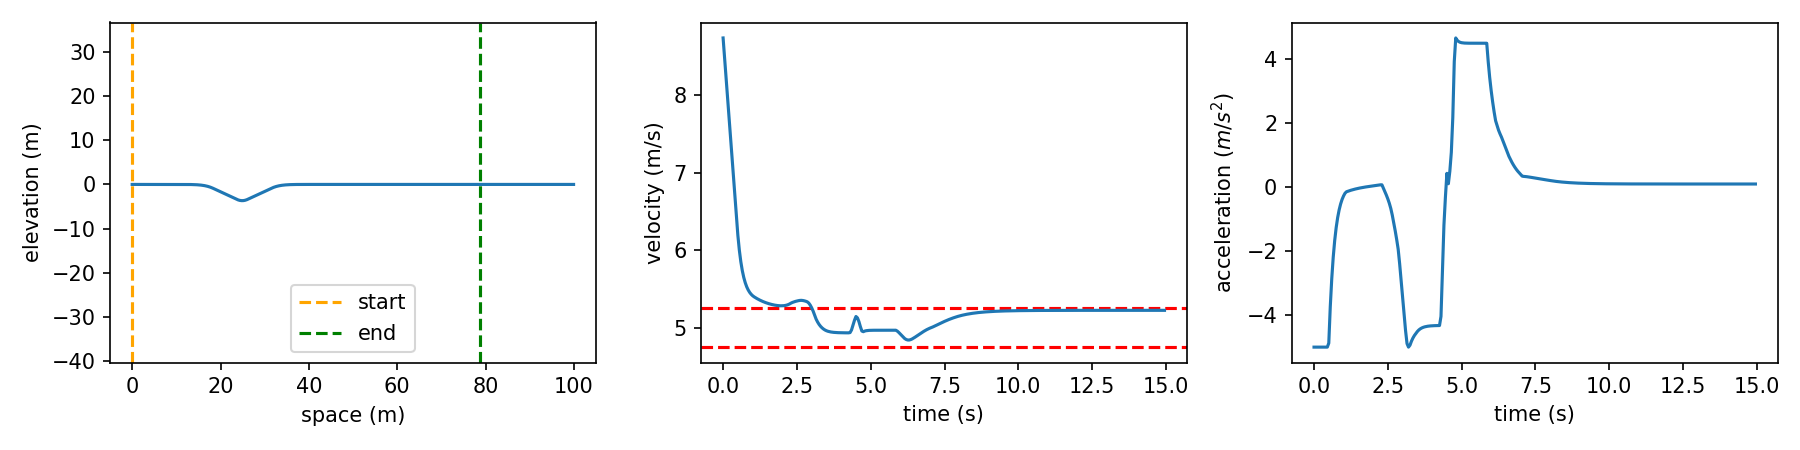
\includegraphics[width=13.8cm, keepaspectratio]{img/5_2_triplot_down.png}
	\caption{Initial configuration: $v_{c0}=8.98 \frac{m}{s}$. In such scenario we see how the defender is able to tackle two problems at the same time: reaching the setpoint and reacting to the change of slope. Still it succeed in managing the situation in a quite stable way.}
    \label{fig:cruise_down}
\end{figure}
In the figures above we can observe how different are the reaction patterns in the case of \textit{attacker}-generated scenario and artificial one.
The \textit{defender} reacts to the landscape generated by the adversarial NN, without noticeable overshoot and handles the situation in a smooth way.
In the case of the artificial hill and valley, instead, it varies more frequently the acceleration patterns even if the profile of the road is much simpler.
In every case, though, the \textit{defender} is able to rapidly reach the desired velocity and keep it. 

In order to perform model comparison and evaluate the performance of the trained model, we ran $10k$ simulations of trajectories.
The following plot shows the percentage of  trajectories that in a given instant was inside the boundary specified by the requirement.

\begin{figure}[H]
	\centering
	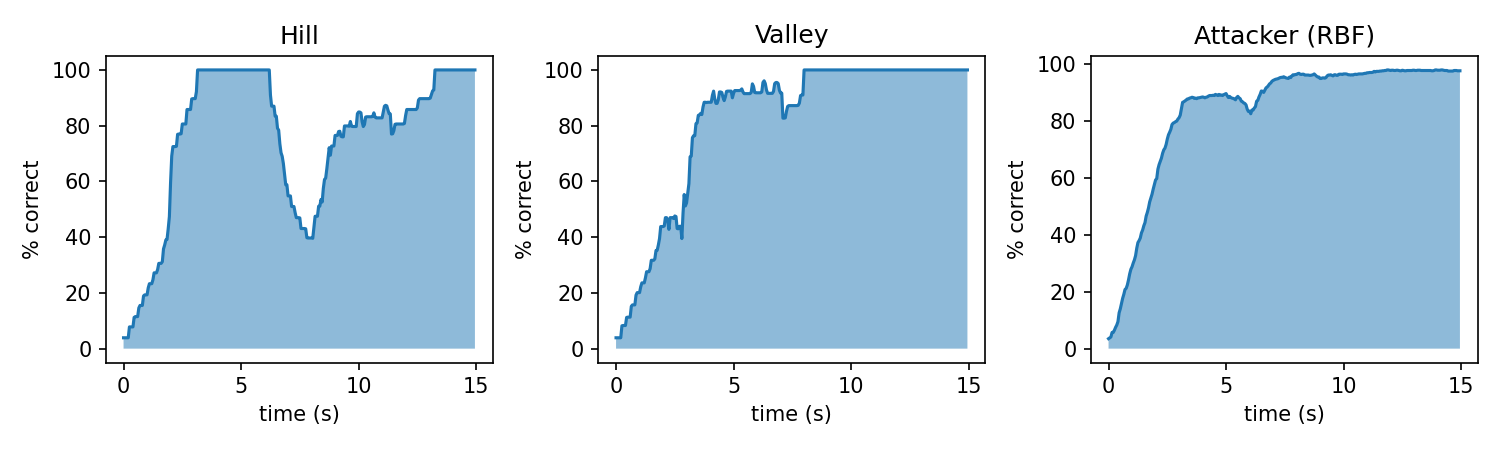
\includegraphics[width=10cm, keepaspectratio]{img/5_2_pct_histogram.png}
	\caption{This plot shows that every single trajectory simulated reached successfully the target velocity, in the end. It is possible to observe how the training on the attacker was very effective. The experience gained in such scenario, though, is less useful in the others, especially in front of sudden change of slope.}
    \label{fig:cruise_pct}
\end{figure}

In the figure \ref{fig:cruise_pct} we can see how successful was the adversarial training for the \textit{defender}: it learnt how to face every possible configuration generated from the attacker.
The smooth growth tells that it can gradually improve the situation over time until it reaches the setpoint.

The first two pictures, instead, show that there is room for improvement for the generalization ability of the \textit{defender}'s NN.
Since the result are already very promising, a better exploration of the space of the road's configuration could lead to perfect results.

\section{Car platooning}
We decided to split the problem of car platooning into a simpler problem of only two cars.
In such simplified setting, we trained both the \textit{attacker} and the \textit{defender} and finally we generalized the behaviour to $n$ cars.
We recall that the problem we want to address is the generation of a safe controller that controls the acceleration of its vehicle in order to keep the distance with the other vehicle inside a given range.

\subsection{Experimental settings}
In the simplified setting of the two cars, we have a \textit{leader} $l$ and a \textit{follower} $f$.
The \textbf{constraint} applied on the CPS described in the chapter before is on the \textit{distance} $d$ between the two vehicles and is $\Phi = \mathcal{G}(d \leq 10 \wedge d \geq 2)$.

Every \textbf{initial configuration} of the experimental runs has been sampled on an \textit{hyper-grid} of three dimensions: leader's velocity $v_{l0}$, leader's position $x_{l0}$ and follower's velocity $v_{f0}$.
The initial velocities $v_{l0}$ and $v_{f0}$ have been sampled among 40 equispaced values in the interval $[0 \frac{m}{s}, 20 \frac{m}{s}]$.
The initial leader's position $x_{l0}$ have been sampled among 15 equispaced values in the interval $[1 \; m,12 \; m]$ while the follower's $x_{f0}$ has been set to $0 \; m$.

The \textbf{attacker}'s architecture is a dense 3-layered NN with 10 neurons per layer.
To each layer has been applied the \textit{Leaky ReLU} activation function \cite{xu2015empirical}.
The dimension of the space to which the noise vector $\textbf{z}$ -- input of the \textit{attacker} NN -- belongs, has been set to $2$.
The \textbf{defender} NN has the same structure of the \textit{attacker} except for the input dimension (does not take as input a noise vector).
In order to compute the trajectory of the actions, both the NNs use a polynomial \textbf{policy function} of order 3.
Therefore, the spaces over which $\textbf{w}_A$ and $\textbf{w}_D$ are defined, have dimension $q = p = 3$.

\begin{figure}[H]
	\centering
	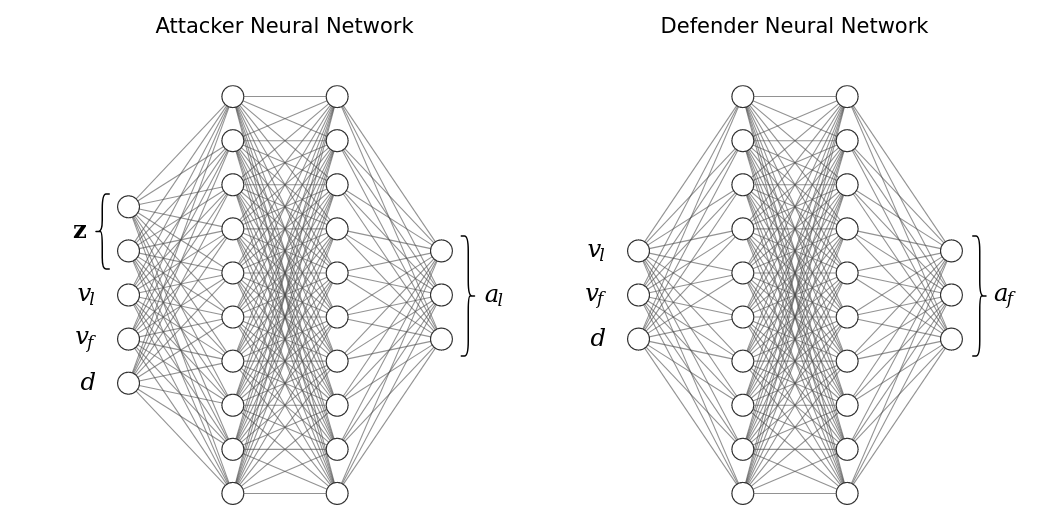
\includegraphics[width=12cm, keepaspectratio]{img/5_3_NNplatooning.png}
	\caption{The architecture used for the the two NN in the car platooning case study. The \textbf{attacker} takes as input the noise vector $\textbf{z}$, the leader's velocity $v_l$, the follower's velocity $v_f$ and their distance $d$. It gives as output the acceleration $a_l$ for the leader's car. The \textbf{defender} takes the same input of the attacker except $\textbf{z}$ and gives as output the follower's acceleration $a_f$.}
\end{figure}

During the training the \textbf{timestep} $\Delta t$ between two time instant has been set to $0.05s$ while the horizon $h$ for each episode was $5s$, 100 timesteps.
The same \textit{timestep} has been used also in the testing.

The training phase lasted $50k$ \textit{cycles} and each \textbf{episode} has been repeated 3 times for the \textit{attacker} and 5 times for the \textit{defender}.

\subsection{Metrics and results}

\subsubsection{One leader and one follower}
We tried many configuration of the hyper-parameters of the model in order to find the ones that were giving the good results presented.

We tested the \textbf{defender-controlled} follower in four different scenarios to check if it was able to adapt effectively to different adversarial strategies.
The first scenario is against the \textit{attacker}, in the second the leader accelerates suddenly, in the third the leader brakes suddenly while in the fourth it accelerates rapidly to brake right after.
For each scenario we show the position of the cars, the relative distance and the acceleration of both.

\begin{figure}[H]
	\centering
	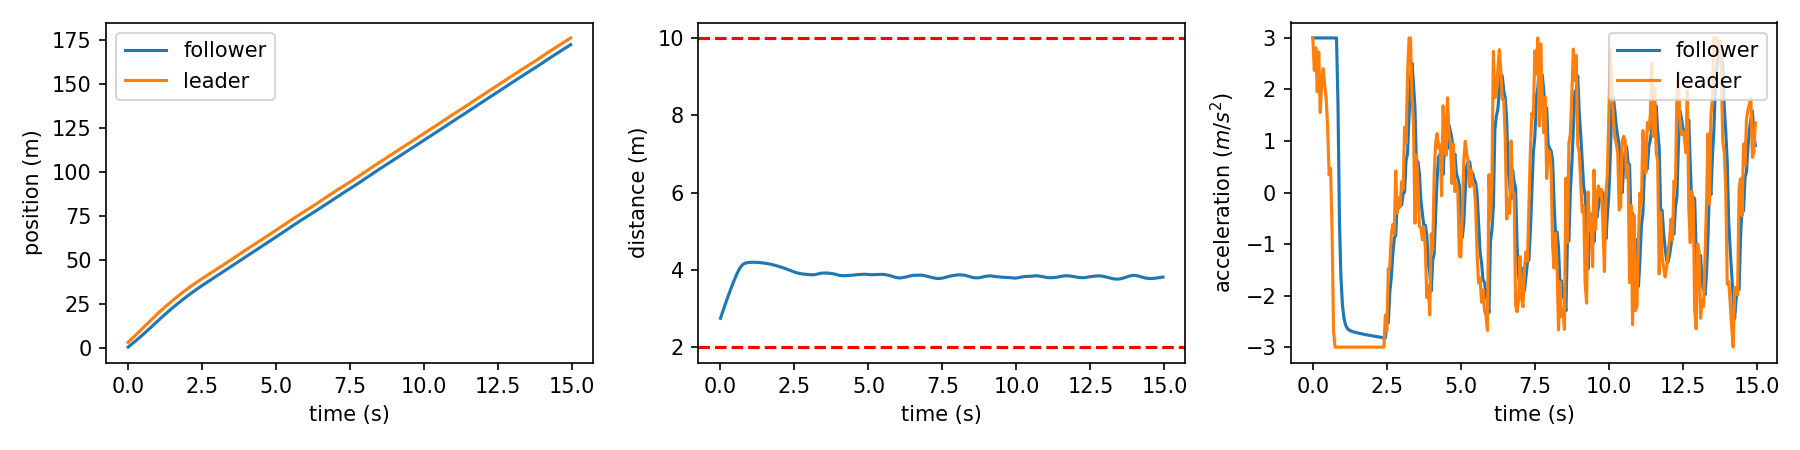
\includegraphics[width=13.8cm, keepaspectratio]{img/5_3_triplot_attacker.png}
	\caption{Initial configuration: $x_{l0}=2.63 \; m$, $v_{l0}=15.58 \frac{m}{s}$, $v_{f0}=13.28 \frac{m}{s}$. We can see how the attacker found the strategy of rapidly accelerating and breaking. The defender, though, succeeds in keeping its distance safe and almost constant over time.}
    \label{fig:single_triplot_attacker}
\end{figure}

\begin{figure}[H]
	\centering
	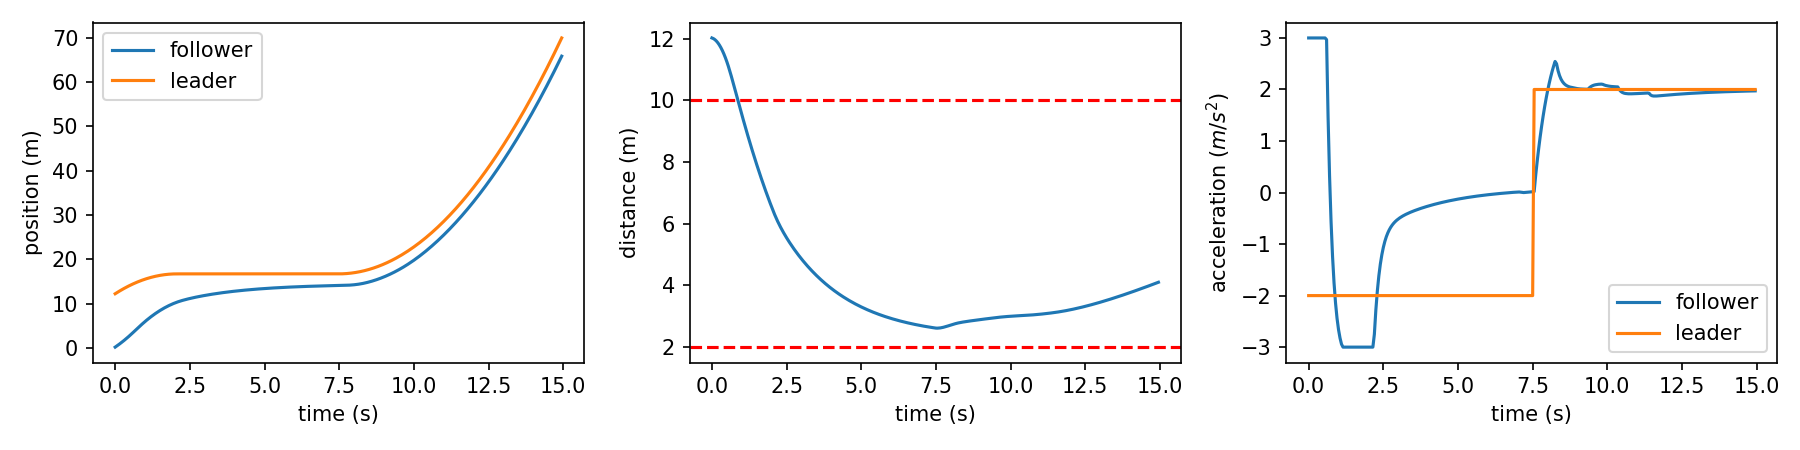
\includegraphics[width=13.8cm, keepaspectratio]{img/5_3_triplot_step_up.png}
	\caption{Initial configuration: $x_{l0}=12.03 \; m$, $v_{l0}=4.49 \frac{m}{s}$, $v_{f0}=4.41 \frac{m}{s}$. In this scenario the defender has the initial disadvantage of being too far from the leader. It safely closes the gap and is able to tolerate the sudden acceleration of the leader.}
    \label{fig:single_triplot_stepup}
\end{figure}

\begin{figure}[H]
	\centering
	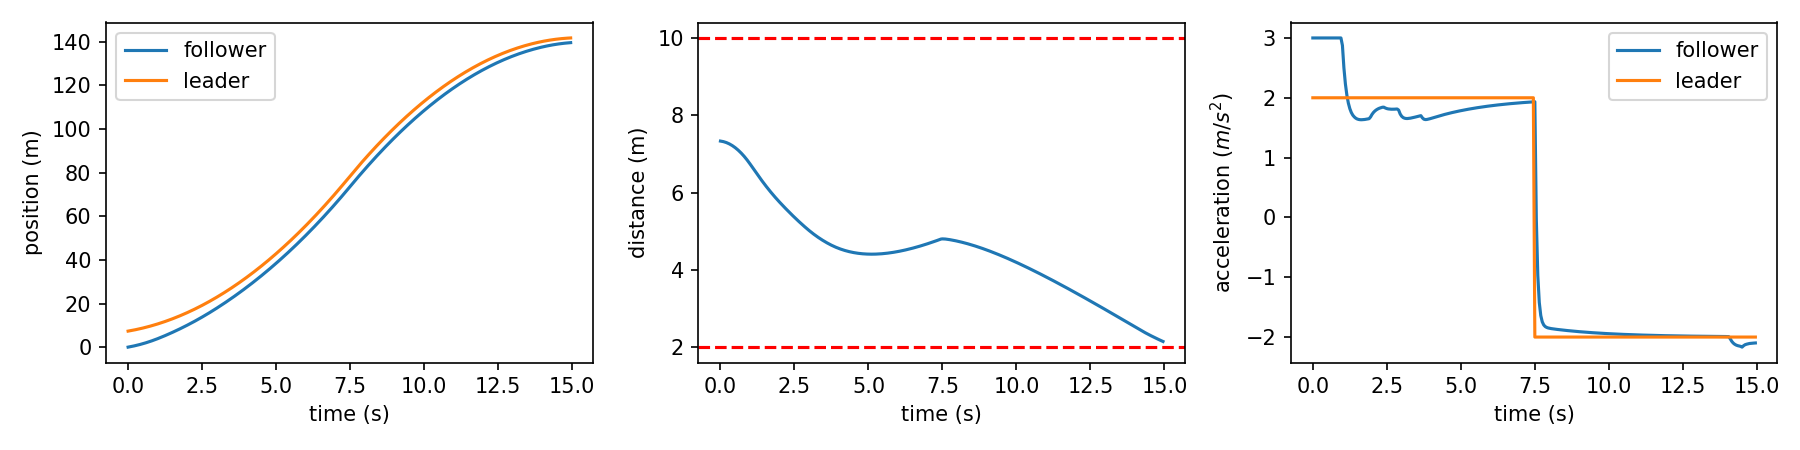
\includegraphics[width=13.8cm, keepaspectratio]{img/5_3_triplot_step_down.png}
	\caption{Initial configuration: $x_{l0}=7.33 \; m$, $v_{l0}=2.19 \frac{m}{s}$, $v_{f0}=2.21 \frac{m}{s}$. In this scenario the defender is able to tolerate quite well the sudden brake since it was keeping the evaluated safety distance.}
    \label{fig:single_triplot_stepdown}
\end{figure}

\begin{figure}[H]
	\centering
	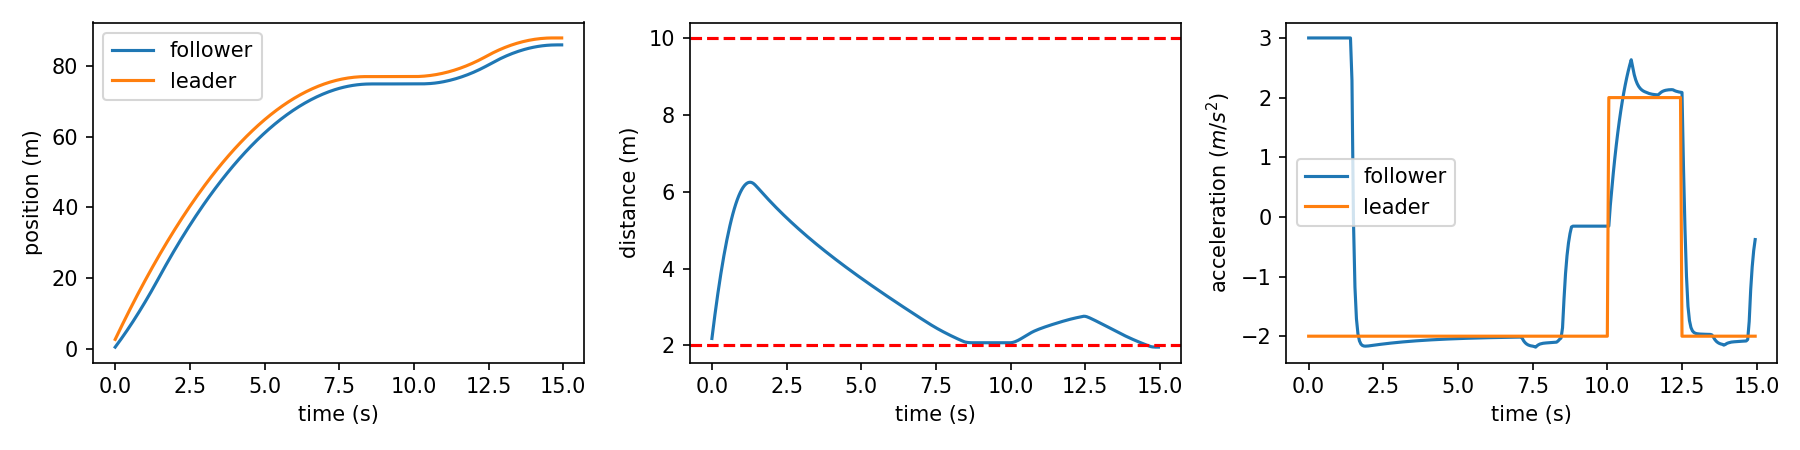
\includegraphics[width=13.8cm, keepaspectratio]{img/5_3_triplot_pulse.png}
	\caption{Initial configuration: $x_{l0}=2.63 \; m$, $v_{l0}=15.58 \frac{m}{s}$, $v_{f0}=13.28 \frac{m}{s}$. In this scenario of sudden acceleration and brake, the defender slowly approaches the opponent until it stops waiting for it to move. It adapts to the opponent behaviour arriving at the minimum allowed distance without violating the constraint.}
    \label{fig:single_triplot_pulse}
\end{figure}

It is possible to notice how well the follower manages the presented corner cases.
In the figure \ref{fig:single_triplot_attacker} we can see how the follower safely keeps an almost steady distance with a leader that behaves in a unpredictable way.
The follower mimics perfectly the acceleration pattern of the leader.
The same happens in the figure \ref{fig:single_triplot_stepdown} where, as soon as the leader suddenly brakes, the follower does the same to keep the safety distance.

In the figure \ref{fig:single_triplot_stepup}, it is interesting to notice how the follower is able to exploit the moments in which the leader is almost static in order to close the initial gap.
Even if the initial condition was not safe, the follower is able to recover from it and maintain the distance between the safety boundaries.

The follower, during the training, has learnt also to halt completely if the leader does so.
Such behaviour is visible in the figure \ref{fig:single_triplot_pulse} in which the follower halts in correspondence with the minimum distance allowed.

Even though the initial configuration plays a crucial role in the controller's safety, it is possible to observe how the NNs develop consistent strategies to solve at best their task.

In order to compare different models and have an estimate of their performances, we ran $10k$ simulation of different trajectories and, for each instant, we computed the percentage of them that was lying inside the given boundaries.
By using this kind of metrics it is possible to have a precise estimate of how well a given model is performing.

\begin{figure}[H]
	\centering
	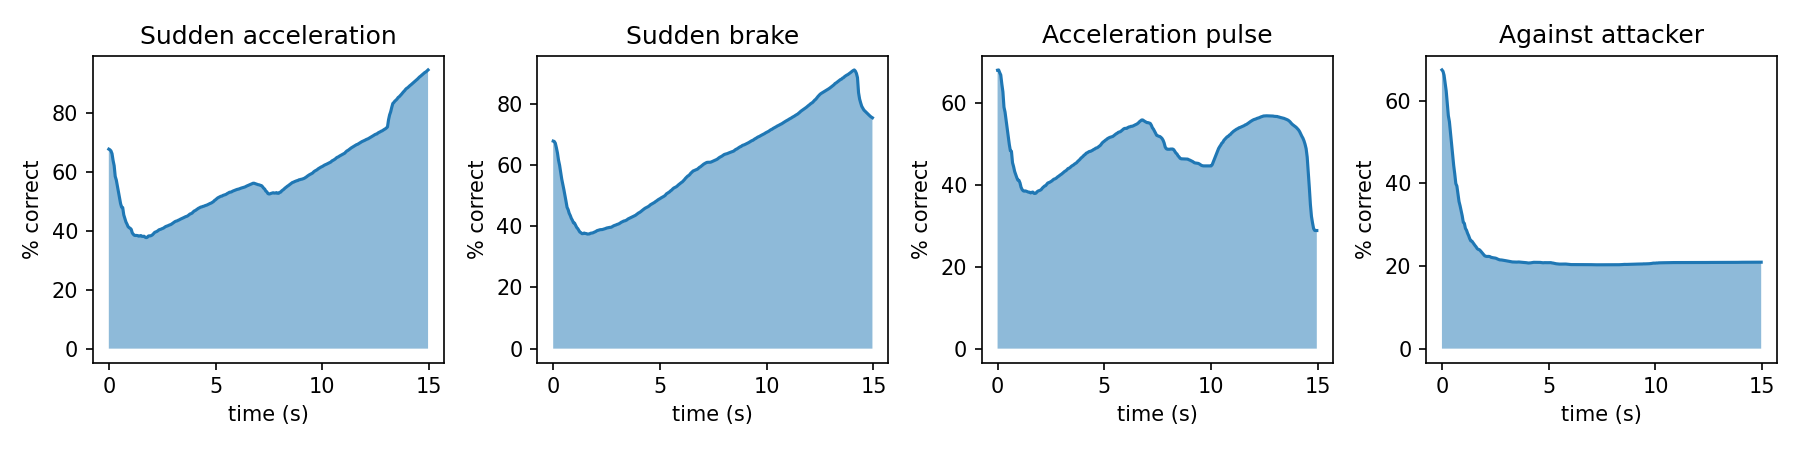
\includegraphics[width=13.8cm, keepaspectratio]{img/5_3_pct_histogram.png}
	\caption{Percentage of correct trajectories for each timestep. We can see that the trained model successfully control over the 80\% of the scenarios of sudden acceleration or brake. It behaves less well with the acceleration pulse and struggle against the attacker's behaviour. It is evident from the plot that in almost 40\% of the cases, the simulation start from forbidden conditions and this should be taken into account to evaluate the model.}
    \label{fig:pct_hist_single}
\end{figure}

It is worth mentioning that the figure \ref{fig:pct_hist_single} shows the results of simulations whose initial conditions have been sampled from the training intervals.
That is to say that, as we can read from the figure, the 30\% of the simulations starts from \textbf{unsafe} initial conditions.

\begin{figure}[H]
	\centering
	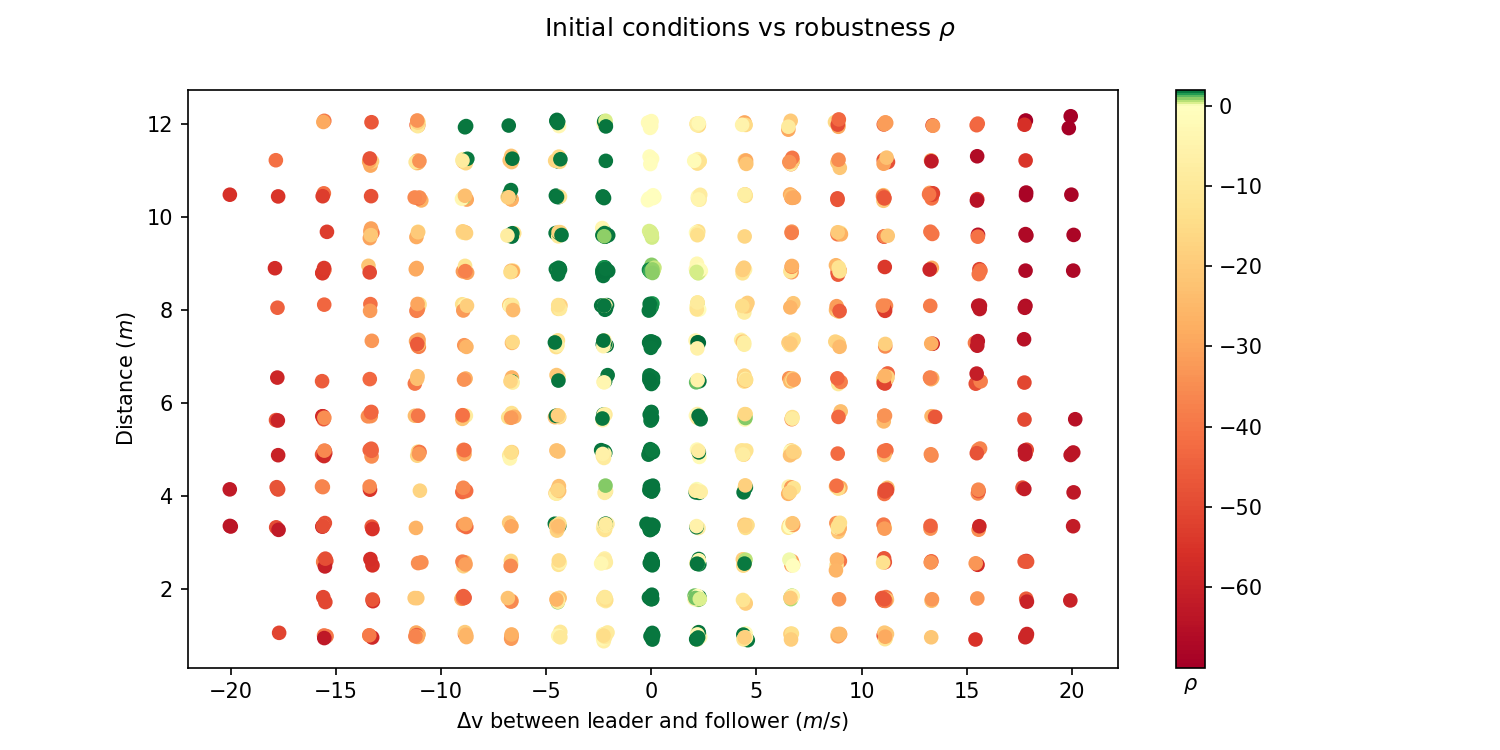
\includegraphics[width=14cm, keepaspectratio]{img/5_3_atk_scatterplot.png}
	\caption{Visualization of the simulations' robustness with respect to the sampled initial conditions. The scenario of the simulations is the one in which the leader is controlled by the attacker NN. This figure shows  the correlation between the initial conditions and the robustness of the defender NN. It is possible to notice how the defender manages very well the cases in which the two cars have similar initial velocity, given that the initial distance is inside the safety range. The  defender can catch up with the attacker even if the latter is further but only if the leader is not going too fast with respect to the follower.}
    \label{fig:atk_scatterplot}
\end{figure}

In the figure \ref{fig:atk_scatterplot} it is possible to notice how the \textit{attacker} is able to exploit favorable scenarios to push the \textit{defender} outside of the safety boundaries.
For instance, if the initial distance is already outside the boundaries and the \textit{attacker} is moving at a considerably different velocity with respect to the follower, it is not possible for the \textit{defender} to get to a safe state (as shown in the figure \ref{fig:atk_scatterplot}).
The \textit{attacker}'s ability to exploit favorable initial conditions could explain the poorer performances of the \textit{defender} in the simulations in which the leader car is controlled by the \textit{attacker} itself.

\subsubsection{One leader and $n$ followers}
Given a solution of the problem for two cars, it was straightforward to extend the application to the platooning of $n$ cars.
The idea is that each car in the line should follow the car in front.
At this stage it does not matter anymore if the car in front is an \textit{attacker} or a \textit{defender}: the aim of each follower is simply to follow.
In such a way it is possible to add an arbitrary number of followers to the line.

The two NNs trained with one leader and only one follower, whose result has been shown above, can be used separately to accomplish such task.
In particular, the only leader of the line will be controlled by the \textit{attacker} NN (or any other arbitrary controller), while all the followers will be controller by a copy of the same \textit{defender} NN.

\begin{figure}[H]
	\centering
	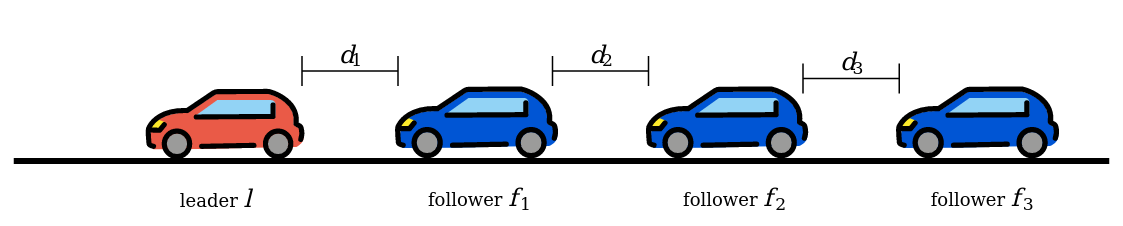
\includegraphics[width=12cm, keepaspectratio]{img/5_3_complete_platooning.png}
	\caption{The complete platooning setting, each car has knowledge of its status and the distance from the car in front.}
\end{figure}

In the tested setting there is only a leader $l$ followed by $3$ followers $f_1$, $f_2$ and $f_3$.
Each follower has to keep the respective distance $d_1$, $d_2$ and $d_3$ with the vehicle in front within the safety range.
In such setting, the leader can be controlled by the \textit{attacker} NN or any adversarial policy.
The follower, instead, are controlled separately by the \textit{defender} NN.

The vehicles start equispaced with an initial distance $d_{init}= d_1 = d_2 = d_3$ drawn from a $\mathcal{U}(1,8)$ distribution.
Similarly, the initial velocity $v_{init}$ of the cars is drawn from a $\mathcal{U}(1,5)$ distribution and is the same for all of them.

We performed the simulations for the whole platoon in the same settings used for the basic case.
The results are shown in the figures from \ref{fig:multi_triplot_attacker} to \ref{fig:multi_triplot_pulse}.
\begin{figure}[H]
	\centering
	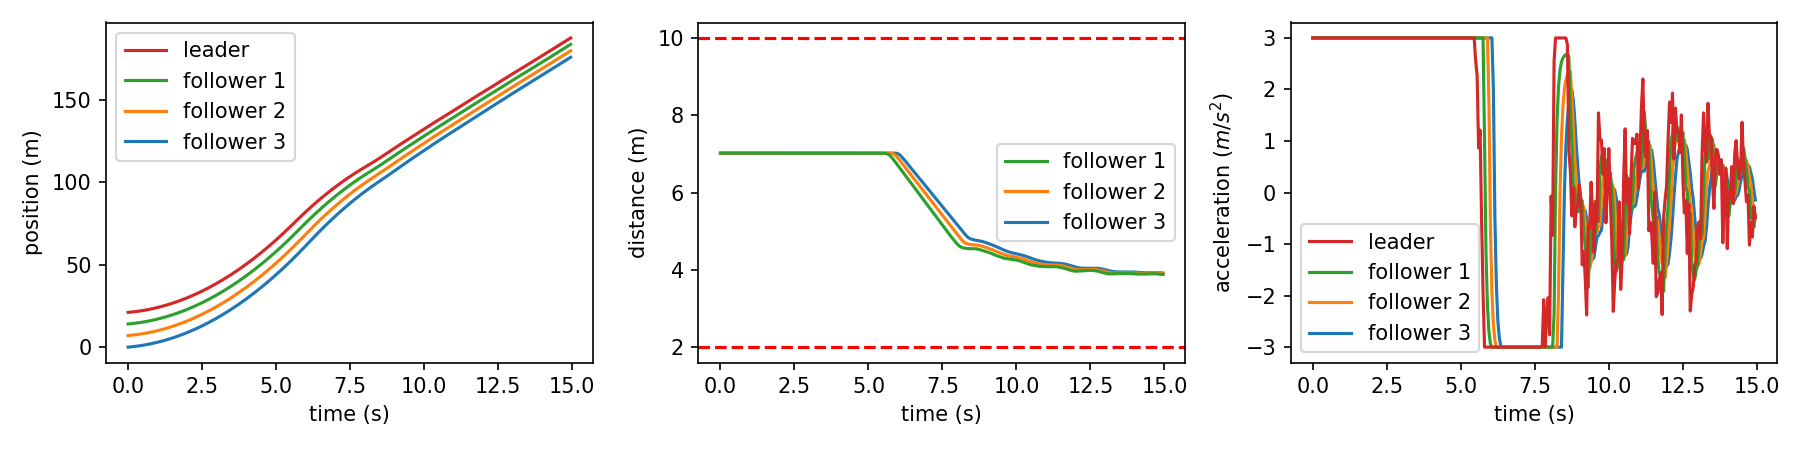
\includegraphics[width=13.8cm, keepaspectratio]{img/5_3_triplot_fullplatooning_attacker.png}
	\caption{Initial configuration: $d_{init}= 7.01\; m$, $v_{init}=1.30 \frac{m}{s}$. We can see how the attacker tries two strategies (sudden brake and rapid acceleration/brake sequence), but the platoon can still manage the situation safely.}
    \label{fig:multi_triplot_attacker}
\end{figure}

\begin{figure}[H]
	\centering
	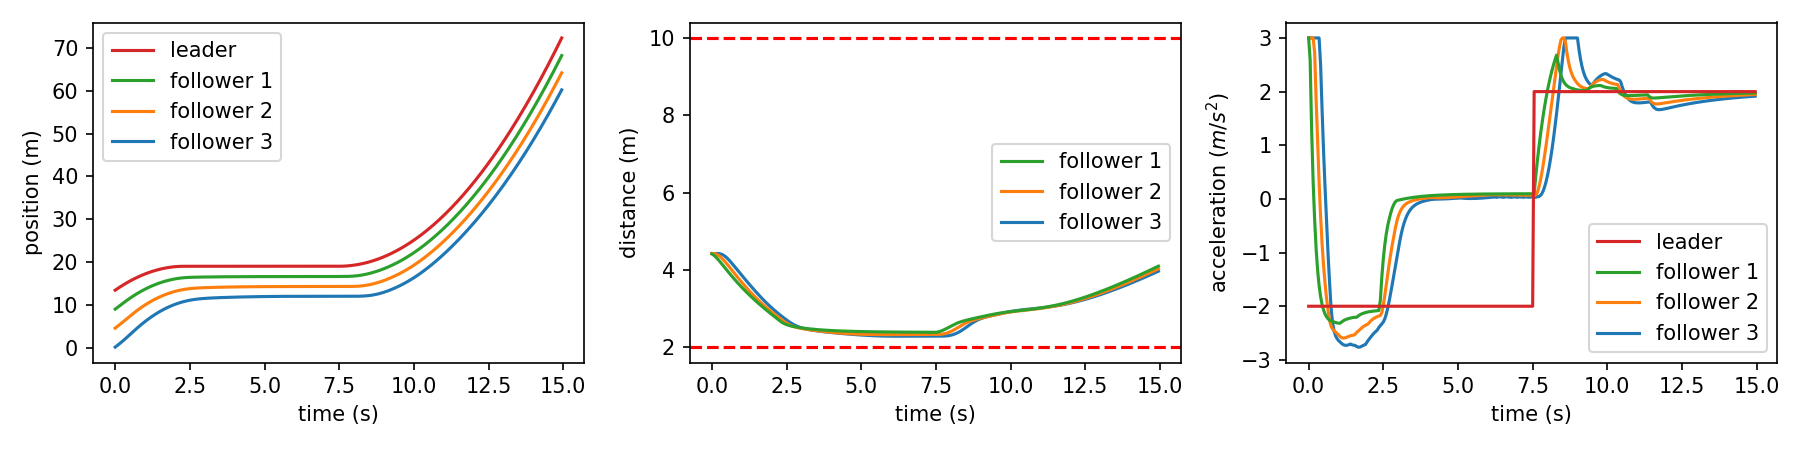
\includegraphics[width=13.8cm, keepaspectratio]{img/5_3_triplot_fullplatooning_stepup.png}
	\caption{Initial configuration: $d_{init}= 4.42\; m$, $v_{init}=4.99 \frac{m}{s}$. It is worth noticing how the whole platoon stops at some point still keeping a safe distance. It restarts right after and hold the safety distance for the rest of the simulation.}
    \label{fig:multi_triplot_stepup}
\end{figure}

\begin{figure}[H]
	\centering
	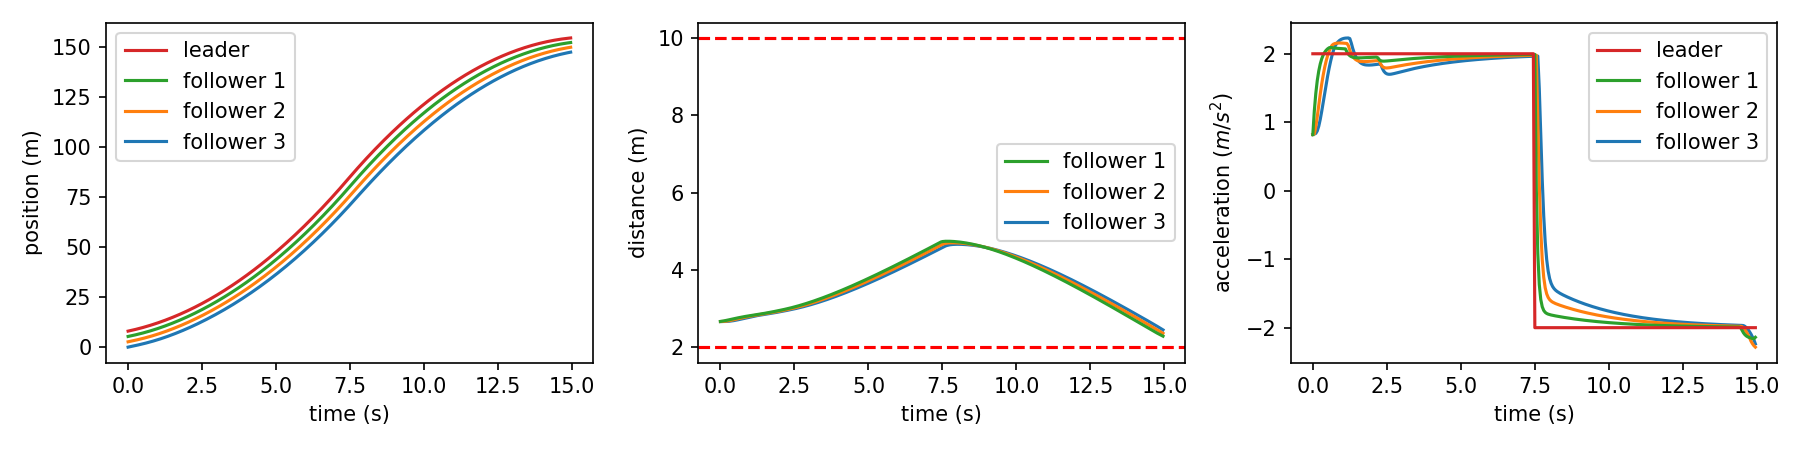
\includegraphics[width=13.8cm, keepaspectratio]{img/5_3_triplot_fullplatooning_stepdown.png}
	\caption{Initial configuration: $d_{init}= 2.66\; m$, $v_{init}=3.01 \frac{m}{s}$. The trajectories are robust despite the sudden brake of the leader.}
    \label{fig:multi_triplot_stepdown}
\end{figure}

\begin{figure}[H]
	\centering
	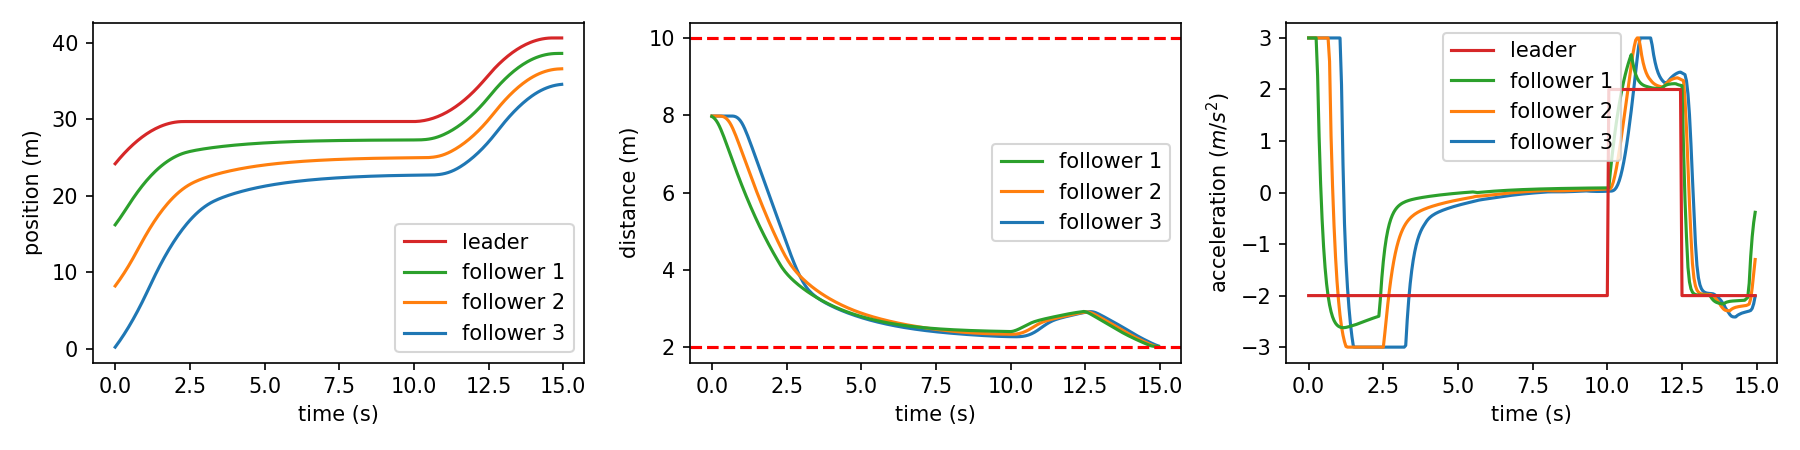
\includegraphics[width=13.8cm, keepaspectratio]{img/5_3_triplot_fullplatooning_pulse.png}
	\caption{Initial configuration: $d_{init}= 7.97\; m$, $v_{init}=4.96 \frac{m}{s}$. The whole platoon reacts interestingly to the sudden changes. As it would happen in the real world, getting further from the head of the platoon, the accelerations changes appear damped and here it is clearly visible.}
    \label{fig:multi_triplot_pulse}
\end{figure}
The platoon's followers behave exactly like the follower of the simple case with one leader and one follower.
This is not surprising since they all use the same NN as controller.
